\documentclass[aspectratio=169,12pt]{beamer}
\usetheme{Madrid}
\usecolortheme{seahorse}
\usepackage{tikz}
\usetikzlibrary{matrix,positioning,arrows.meta,decorations.pathreplacing,fit,calc,shapes}
\usepackage{amsmath,amssymb}
\usepackage[T1]{fontenc}

\newcommand{\Oh}{\mathcal{O}}

\setbeamertemplate{navigation symbols}{}
\setbeamertemplate{footline}[frame number]

\title{Dynamic Data Structures\\for Twin-Ordered Matrices}
\author{B.~Bosek, J.~Czy\.zewska, E.~Kipouridis,\\W.~Nadara, M.~Pilipczuk, K.~W\k{e}grzycki, A.~Zych-Pawlewicz}
\institute{Jagiellonian University $\cdot$ University of Warsaw $\cdot$ MPI Informatics}
\date{LATIN 2026}

\begin{document}

% ============ SLIDE 1 ============
\begin{frame}
\titlepage
\begin{tikzpicture}[remember picture,overlay]
\node[opacity=0.15,anchor=south east] at (current page.south east) {
\begin{tikzpicture}
\matrix[matrix of nodes, nodes={minimum size=6mm, draw, thin, font=\tiny},
  column sep=-\pgflinewidth, row sep=-\pgflinewidth]{
0 & 1 & 1 & 1 & 1 \\
0 & 0 & 0 & 0 & 1 \\
1 & 1 & 1 & 0 & 0 \\
1 & 1 & 1 & 0 & 1 \\
1 & 0 & 0 & 1 & 1 \\
};
\end{tikzpicture}
};
\end{tikzpicture}
\end{frame}

% ============ SLIDE 2 ============
\begin{frame}{Twin-width: the big picture}
\begin{columns}
\begin{column}{0.45\textwidth}
\textbf{Twin-width} [Bonnet, Kim, Thomass\'e, Watrigant 2022]

\medskip
A unifying structural parameter for:
\begin{itemize}
\item graphs (sparse \& dense)
\item matrices
\item permutations
\end{itemize}
\end{column}
\begin{column}{0.55\textwidth}
\centering
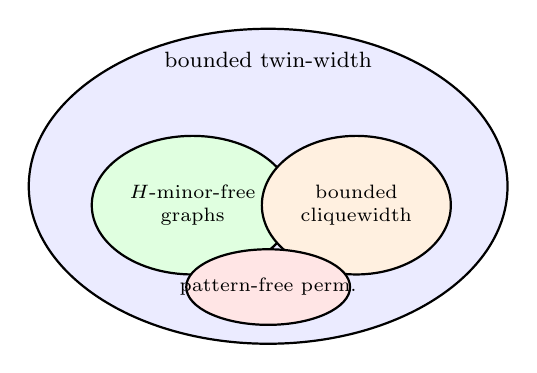
\begin{tikzpicture}[scale=0.8]
  \draw[thick,fill=blue!8] (0,0) ellipse (3.8 and 2.5);
  \node at (0,2) {\footnotesize bounded twin-width};
  \draw[thick,fill=green!12] (-1.2,-0.3) ellipse (1.6 and 1.1);
  \node[font=\scriptsize,align=center] at (-1.2,-0.3) {$H$-minor-free\\graphs};
  \draw[thick,fill=orange!12] (1.4,-0.3) ellipse (1.5 and 1.1);
  \node[font=\scriptsize,align=center] at (1.4,-0.3) {bounded\\cliquewidth};
  \draw[thick,fill=red!10] (0,-1.6) ellipse (1.3 and 0.6);
  \node[font=\scriptsize] at (0,-1.6) {pattern-free perm.};
\end{tikzpicture}
\end{column}
\end{columns}
\end{frame}

% ============ SLIDE 3 ============
\begin{frame}{Contraction sequence: idea}
\centering
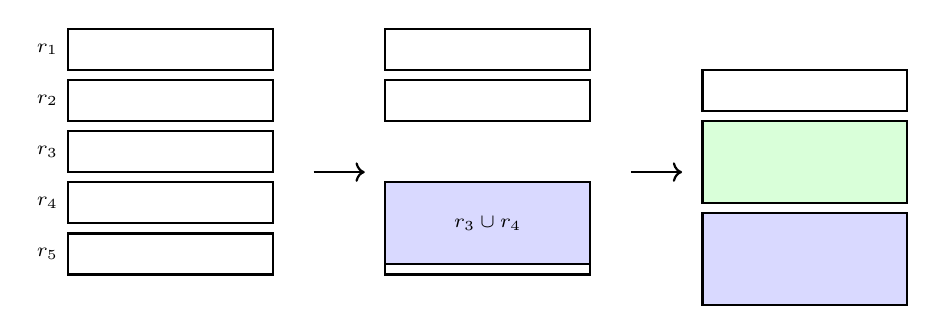
\begin{tikzpicture}[scale=0.65]
% Step 1: 5 separate rows
\foreach \i in {1,...,5} {
  \draw[thick] (0,6-\i) rectangle +(4,0.8);
  \node[font=\scriptsize] at (-0.4,6-\i+0.4) {$r_\i$};
}
\draw[->,thick] (4.8,3) -- (5.8,3);
% Step 2: merge r3,r4
\foreach \i in {1,2,5} {
  \draw[thick] (6.2,6-\i) rectangle +(4,0.8);
}
\draw[thick,fill=blue!15] (6.2,1.2) rectangle +(4,1.6);
\node[font=\scriptsize] at (8.2,2) {$r_3 \cup r_4$};
\draw[->,thick] (11,3) -- (12,3);
% Step 3: further merge
\draw[thick] (12.4,4.2) rectangle +(4,0.8);
\draw[thick,fill=green!15] (12.4,2.4) rectangle +(4,1.6);
\draw[thick,fill=blue!15] (12.4,0.4) rectangle +(4,1.8);
\end{tikzpicture}

\medskip
Iteratively merge consecutive row/column blocks.

At each step: $\leq d$ non-constant zones per block.
\end{frame}

% ============ SLIDE 4 ============
\begin{frame}{Contraction sequence: example ($d=2$)}
\centering
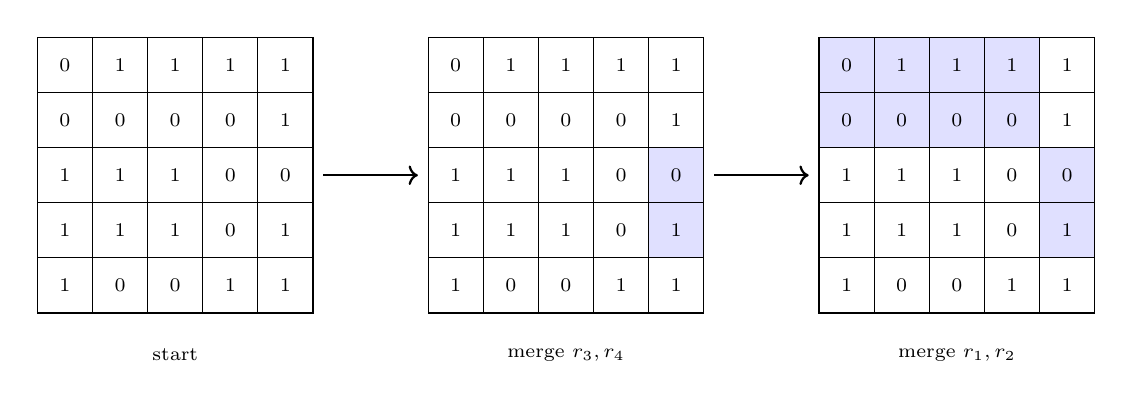
\begin{tikzpicture}[scale=0.58]
\tikzset{cell/.style={minimum size=7mm,draw,thin,font=\scriptsize,inner sep=0pt}}
\tikzset{ncell/.style={cell,fill=blue!12}}
% Matrix step 1
\matrix (m1) [matrix of nodes, nodes={cell}, column sep=-\pgflinewidth, row sep=-\pgflinewidth] {
0 & 1 & 1 & 1 & 1 \\
0 & 0 & 0 & 0 & 1 \\
1 & 1 & 1 & 0 & 0 \\
1 & 1 & 1 & 0 & 1 \\
1 & 0 & 0 & 1 & 1 \\
};
\node[below=2mm,font=\scriptsize] at (m1.south) {start};

% Matrix step 2: merge rows 3,4
\matrix (m2) [matrix of nodes, nodes={cell}, column sep=-\pgflinewidth, row sep=-\pgflinewidth,
  right=12mm of m1] {
0 & 1 & 1 & 1 & 1 \\
0 & 0 & 0 & 0 & 1 \\
1 & 1 & 1 & 0 & |[ncell]| 0 \\
1 & 1 & 1 & 0 & |[ncell]| 1 \\
1 & 0 & 0 & 1 & 1 \\
};
\node[below=2mm,font=\scriptsize] at (m2.south) {merge $r_3,r_4$};

% Matrix step 3: merge cols 2,3
\matrix (m3) [matrix of nodes, nodes={cell}, column sep=-\pgflinewidth, row sep=-\pgflinewidth,
  right=12mm of m2] {
|[ncell]| 0 & |[ncell]| 1 & |[ncell]| 1 & |[ncell]| 1 & 1 \\
|[ncell]| 0 & |[ncell]| 0 & |[ncell]| 0 & |[ncell]| 0 & 1 \\
1 & 1 & 1 & 0 & |[ncell]| 0 \\
1 & 1 & 1 & 0 & |[ncell]| 1 \\
1 & 0 & 0 & 1 & 1 \\
};
\node[below=2mm,font=\scriptsize] at (m3.south) {merge $r_1,r_2$};

\draw[->,thick] (m1.east) -- (m2.west);
\draw[->,thick] (m2.east) -- (m3.west);
\end{tikzpicture}

\bigskip
{\color{blue!60!black} Colored} = non-constant zones.

Each block has $\leq 2$ non-constant zones $\Rightarrow$ width $2$.
\end{frame}

% ============ SLIDE 5 ============
\begin{frame}{$d$-twin-ordered vs twin-width $\leq d$}
\centering
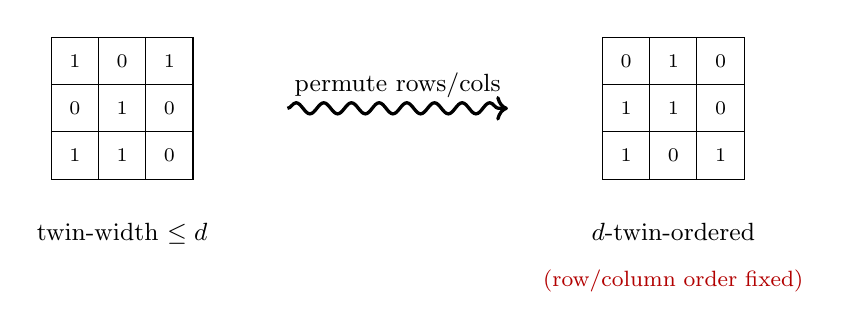
\begin{tikzpicture}[scale=0.7]
% Left: arbitrary matrix
\matrix (m1) [matrix of nodes, nodes={minimum size=6mm,draw,thin,font=\scriptsize},
  column sep=-\pgflinewidth, row sep=-\pgflinewidth] {
1 & 0 & 1 \\
0 & 1 & 0 \\
1 & 1 & 0 \\
};
\node[below=3mm,font=\small] at (m1.south) {twin-width $\leq d$};

\draw[->,very thick,decorate,decoration={snake,amplitude=2pt,segment length=10pt}] (3,0) -- node[above,font=\small]{permute rows/cols} (7,0);

% Right: ordered matrix
\matrix (m2) [matrix of nodes, nodes={minimum size=6mm,draw,thin,font=\scriptsize},
  column sep=-\pgflinewidth, row sep=-\pgflinewidth] at (10,0) {
0 & 1 & 0 \\
1 & 1 & 0 \\
1 & 0 & 1 \\
};
\node[below=3mm,font=\small] at (m2.south) {$d$-twin-ordered};
\node[below=9mm,font=\footnotesize,red!70!black] at (m2.south) {(row/column order fixed)};
\end{tikzpicture}

\bigskip
\textbf{We work with:} $d$-twin-ordered matrices (order is fixed).
\end{frame}

% ============ SLIDE 6 ============
\begin{frame}{Main theorem}
\begin{block}{Theorem (Main Result)}
Let $d \in \mathbb{N}$, $M \in \{0,1\}^{n \times n}$ be $d$-twin-ordered at every moment. There exists a dynamic data structure using $\Oh_d(n)$ memory supporting:
\begin{itemize}
\item $\mathtt{Init}(n, \mathcal{K})$: initialize in $\Oh_d((n+|\mathcal{K}|)\log\log n)$ time
\item $\mathtt{QueryBit}(i,j)$: return $M[i,j]$ in $\Oh(\log\log n)$ exp.\ w.c.\ time
\item $\mathtt{Update}(i,j)$: flip $M[i,j]$ in $\Oh(\log\log n)$ exp.\ w.c.\ time
\end{itemize}
\end{block}

\centering
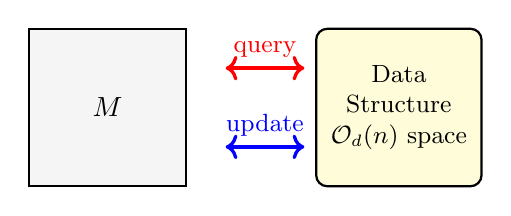
\begin{tikzpicture}[scale=0.5]
\draw[thick,fill=gray!8] (0,0) rectangle (4,4);
\node at (2,2) {$M$};
\draw[<->,red,very thick] (5,3) -- node[above,font=\small]{query} (7,3);
\draw[<->,blue,very thick] (5,1) -- node[above,font=\small]{update} (7,1);
\draw[thick,fill=yellow!15,rounded corners] (7.3,0) rectangle (11.5,4);
\node[align=center,font=\small] at (9.4,2) {Data\\Structure\\$\Oh_d(n)$ space};
\end{tikzpicture}
\end{frame}

% ============ SLIDE 7 ============
\begin{frame}{Context: prior work}
\centering
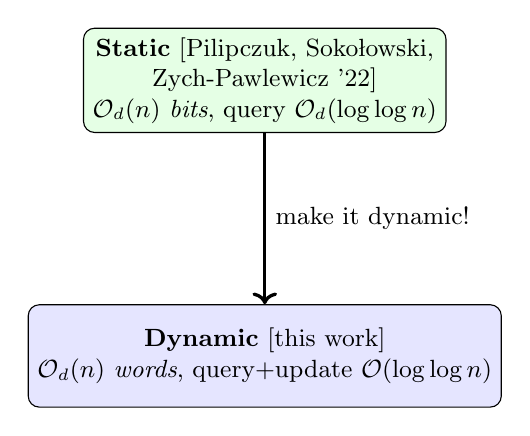
\begin{tikzpicture}[
  box/.style={draw,rounded corners,minimum width=4.5cm,minimum height=1.3cm,align=center,font=\small}
]
\node[box,fill=green!10] (static) at (0,2) {\textbf{Static} [Pilipczuk, Sokołowski,\\Zych-Pawlewicz '22]\\$\Oh_d(n)$ \emph{bits}, query $\Oh_d(\log\log n)$};
\node[box,fill=blue!10] (dynamic) at (0,-1.5) {\textbf{Dynamic} [this work]\\$\Oh_d(n)$ \emph{words}, query+update $\Oh(\log\log n)$};
\draw[->,very thick] (static) -- node[right,font=\small]{make it dynamic!} (dynamic);
\end{tikzpicture}
\end{frame}

% ============ SLIDE 8 ============
\begin{frame}{Slabs and slab decompositions}
\begin{columns}
\begin{column}{0.45\textwidth}
A \textbf{slab} = all-ones rectangle $M[[a,b],[c,d]]$.

\medskip
A \textbf{slab decomposition} = pairwise disjoint slabs covering all $1$s.
\end{column}
\begin{column}{0.55\textwidth}
\centering
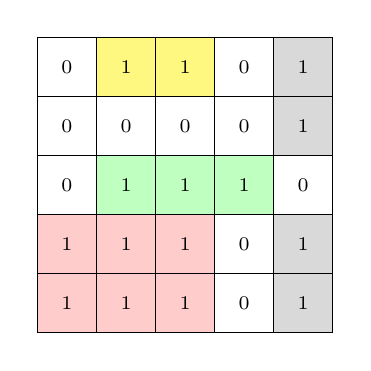
\begin{tikzpicture}[scale=0.7]
\tikzset{cell/.style={minimum size=7.5mm,draw,thin,font=\scriptsize,inner sep=0pt}}
\matrix (m) [matrix of nodes, nodes={cell}, column sep=-\pgflinewidth, row sep=-\pgflinewidth] {
0 & |[fill=yellow!50]| 1 & |[fill=yellow!50]| 1 & 0 & |[fill=gray!30]| 1 \\
0 & 0 & 0 & 0 & |[fill=gray!30]| 1 \\
0 & |[fill=green!25]| 1 & |[fill=green!25]| 1 & |[fill=green!25]| 1 & 0 \\
|[fill=red!20]| 1 & |[fill=red!20]| 1 & |[fill=red!20]| 1 & 0 & |[fill=black!15]| 1 \\
|[fill=red!20]| 1 & |[fill=red!20]| 1 & |[fill=red!20]| 1 & 0 & |[fill=black!15]| 1 \\
};
\end{tikzpicture}

\smallskip
{\scriptsize 5 slabs shown in distinct colors}
\end{column}
\end{columns}
\end{frame}

% ============ SLIDE 9 ============
\begin{frame}{Key structural fact: few slabs suffice}

\begin{block}{Lemma (from [PSZ '22])}
A $d$-twin-ordered $n \times n$ matrix admits a slab decomposition $\mathcal{K}$ with $|\mathcal{K}| \leq d(2n-2)+1$.
\end{block}

\centering
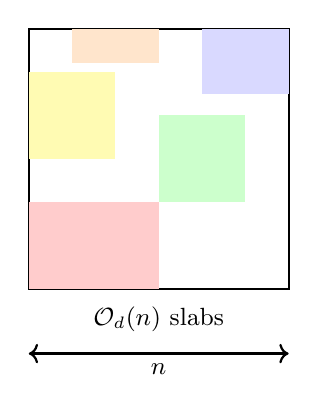
\begin{tikzpicture}[scale=0.55]
\draw[thick] (0,0) rectangle (6,6);
\fill[red!20] (0,0) rectangle (3,2);
\fill[yellow!30] (0,3) rectangle (2,5);
\fill[green!20] (3,2) rectangle (5,4);
\fill[blue!15] (4,4.5) rectangle (6,6);
\fill[orange!20] (1,5.2) rectangle (3,6);
\node[font=\small] at (3,-0.7) {$\Oh_d(n)$ slabs};
\draw[<->,thick] (0,-1.5) -- node[below,font=\small]{$n$} (6,-1.5);
\end{tikzpicture}
\end{frame}

% ============ SLIDE 10 ============
\begin{frame}{Corners in twin-ordered matrices}
\begin{columns}
\begin{column}{0.5\textwidth}
A \textbf{corner} = a $2\times 2$ zone with both rows different and both columns different.

\begin{block}{Lemma}
A $d$-twin-ordered $n \times n$ matrix has $\leq f_d \cdot (n+2) \in \Oh_d(n)$ corners.
\end{block}
\end{column}
\begin{column}{0.5\textwidth}
\centering
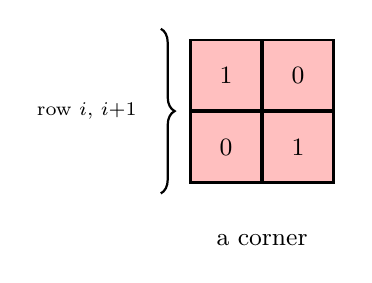
\begin{tikzpicture}[scale=0.8]
\tikzset{cell/.style={minimum size=9mm,draw,thick,font=\small,inner sep=0pt}}
\matrix (m) [matrix of nodes, nodes={cell}, column sep=-\pgflinewidth, row sep=-\pgflinewidth] {
|[fill=red!25]| 1 & |[fill=red!25]| 0 \\
|[fill=red!25]| 0 & |[fill=red!25]| 1 \\
};
\node[below=4mm,font=\small] at (m.south) {a corner};
\draw[decorate,decoration={brace,amplitude=5pt},thick] ([xshift=-3mm]m.north west) -- ([xshift=-3mm]m.south west) node[midway,left=5pt,font=\scriptsize]{row $i$, $i{+}1$};
\end{tikzpicture}
\end{column}
\end{columns}
\end{frame}

% ============ SLIDE 11 ============
\begin{frame}{Proof roadmap}
\centering
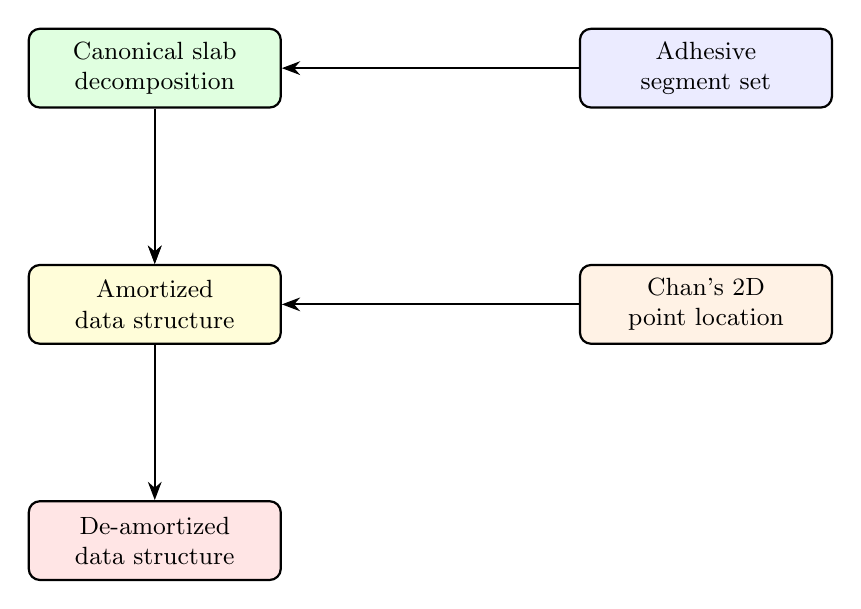
\begin{tikzpicture}[
  block/.style={draw,rounded corners,minimum width=3.2cm,minimum height=1cm,align=center,font=\small,thick},
  arr/.style={->,>=Stealth,thick}
]
\node[block,fill=green!12] (canon) at (0,3) {Canonical slab\\decomposition};
\node[block,fill=yellow!15] (amort) at (0,0) {Amortized\\data structure};
\node[block,fill=red!10] (deamort) at (0,-3) {De-amortized\\data structure};

\node[block,fill=blue!8] (veb) at (7,3) {Adhesive\\segment set};
\node[block,fill=orange!10] (chan) at (7,0) {Chan's 2D\\point location};

\draw[arr] (canon) -- (amort);
\draw[arr] (amort) -- (deamort);
\draw[arr] (veb) -- (canon);
\draw[arr] (chan) -- (amort);
\draw[arr] (canon) -- (amort);
\end{tikzpicture}
\end{frame}

% ============ SLIDE 12 ============
\begin{frame}{Tool: van Emde Boas trees}
\centering
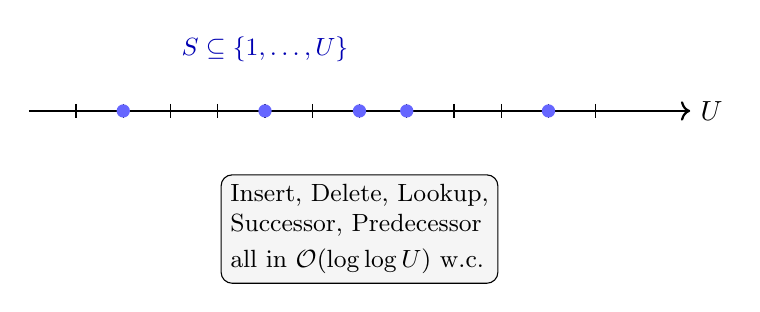
\begin{tikzpicture}[scale=0.6]
% Number line
\draw[thick,->] (0,0) -- (14,0) node[right]{$U$};
\foreach \x in {1,...,12} {
  \draw (\x,0.15) -- (\x,-0.15);
}
% Stored keys
\foreach \x in {2,5,7,8,11} {
  \fill[blue!60] (\x,0) circle (4pt);
}
\node[above=5mm,font=\small,blue!70!black] at (5,0) {$S \subseteq \{1,\ldots,U\}$};

% Operations box
\node[draw,rounded corners,fill=gray!8,align=left,font=\small] at (7,-2.5) {
  Insert, Delete, Lookup,\\
  Successor, Predecessor\\[2pt]
  all in $\Oh(\log\log U)$ w.c.
};
\end{tikzpicture}
\end{frame}

% ============ SLIDE 13 ============
\begin{frame}{Tool: adhesive segment set}
\centering
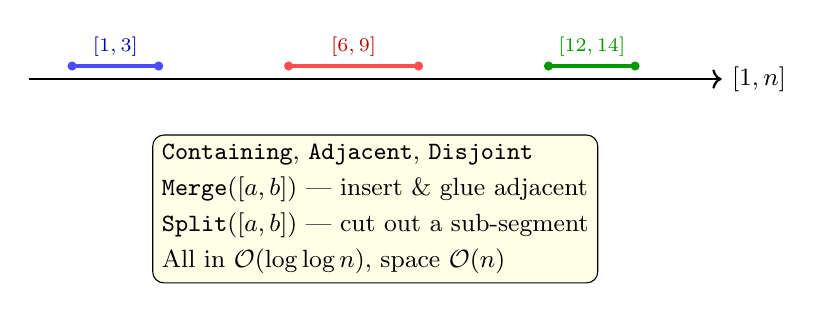
\begin{tikzpicture}[scale=0.55]
\draw[thick,->] (0,0) -- (16,0) node[right,font=\small]{$[1,n]$};
% Segments
\draw[very thick,blue!70] (1,0.3) -- (3,0.3);
\fill[blue!70] (1,0.3) circle (3pt); \fill[blue!70] (3,0.3) circle (3pt);
\node[above,font=\scriptsize,blue!70!black] at (2,0.3) {$[1,3]$};

\draw[very thick,red!70] (6,0.3) -- (9,0.3);
\fill[red!70] (6,0.3) circle (3pt); \fill[red!70] (9,0.3) circle (3pt);
\node[above,font=\scriptsize,red!70!black] at (7.5,0.3) {$[6,9]$};

\draw[very thick,green!60!black] (12,0.3) -- (14,0.3);
\fill[green!60!black] (12,0.3) circle (3pt); \fill[green!60!black] (14,0.3) circle (3pt);
\node[above,font=\scriptsize,green!60!black] at (13,0.3) {$[12,14]$};

% Operations
\node[draw,rounded corners,fill=yellow!10,align=left,font=\small] at (8,-3) {
  $\mathtt{Containing}$, $\mathtt{Adjacent}$, $\mathtt{Disjoint}$\\[2pt]
  $\mathtt{Merge}([a,b])$ --- insert \& glue adjacent\\[2pt]
  $\mathtt{Split}([a,b])$ --- cut out a sub-segment\\[2pt]
  All in $\Oh(\log\log n)$, space $\Oh(n)$
};
\end{tikzpicture}
\end{frame}

% ============ SLIDE 14 ============
\begin{frame}{Merge operation illustrated}
\centering
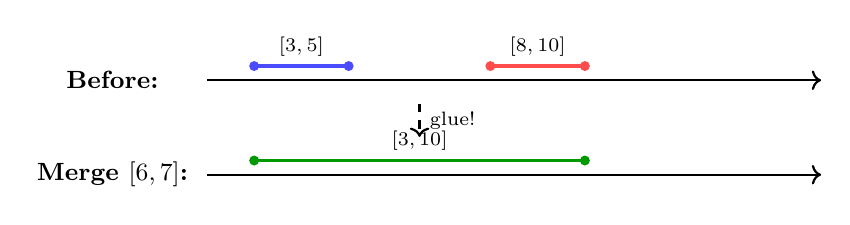
\begin{tikzpicture}[scale=0.6]
% Before
\node[font=\small\bfseries] at (0,2.5) {Before:};
\draw[thick,->] (2,2.5) -- (15,2.5);
\draw[very thick,blue!70] (3,2.8) -- (5,2.8);
\fill[blue!70] (3,2.8) circle (3pt); \fill[blue!70] (5,2.8) circle (3pt);
\node[above,font=\scriptsize] at (4,2.8) {$[3,5]$};
\draw[very thick,red!70] (8,2.8) -- (10,2.8);
\fill[red!70] (8,2.8) circle (3pt); \fill[red!70] (10,2.8) circle (3pt);
\node[above,font=\scriptsize] at (9,2.8) {$[8,10]$};

% Merge [6,7]
\node[font=\small\bfseries] at (0,0.5) {Merge $[6,7]$:};
\draw[thick,->] (2,0.5) -- (15,0.5);
\draw[very thick,green!60!black] (3,0.8) -- (10,0.8);
\fill[green!60!black] (3,0.8) circle (3pt); \fill[green!60!black] (10,0.8) circle (3pt);
\node[above,font=\scriptsize] at (6.5,0.8) {$[3,10]$};

\draw[->,thick,dashed] (6.5,2) -- (6.5,1.3) node[midway,right,font=\scriptsize]{glue!};
\end{tikzpicture}
\end{frame}

% ============ SLIDE 15 ============
\begin{frame}{Strips and siblings}
\begin{columns}
\begin{column}{0.45\textwidth}
An \textbf{$i$-strip}: maximal all-ones segment in column $i$.

\medskip
Two strips in columns $i, j$ are \textbf{siblings} if identical strips exist in every column between them.
\end{column}
\begin{column}{0.55\textwidth}
\centering
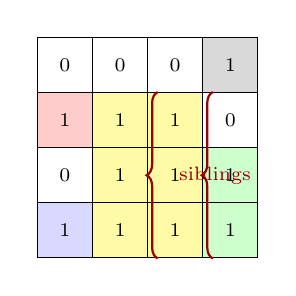
\begin{tikzpicture}[scale=0.6]
\tikzset{cell/.style={minimum size=7mm,draw,thin,font=\scriptsize,inner sep=0pt}}
\matrix (m) [matrix of nodes, nodes={cell}, column sep=-\pgflinewidth, row sep=-\pgflinewidth] {
0 & 0 & 0 & |[fill=black!15]| 1 \\
|[fill=red!20]| 1 & |[fill=yellow!35]| 1 & |[fill=yellow!35]| 1 & 0 \\
0 & |[fill=yellow!35]| 1 & |[fill=yellow!35]| 1 & |[fill=green!20]| 1 \\
|[fill=blue!15]| 1 & |[fill=yellow!35]| 1 & |[fill=yellow!35]| 1 & |[fill=green!20]| 1 \\
};
\draw[decorate,decoration={brace,amplitude=4pt,mirror},thick,red!60!black]
  ([xshift=2mm]m-2-2.north east) -- ([xshift=2mm]m-4-2.south east)
  node[midway,right=4pt,font=\scriptsize]{siblings};
\draw[decorate,decoration={brace,amplitude=4pt,mirror},thick,red!60!black]
  ([xshift=2mm]m-2-3.north east) -- ([xshift=2mm]m-4-3.south east);
\end{tikzpicture}
\end{column}
\end{columns}
\end{frame}

% ============ SLIDE 16 ============
\begin{frame}{Canonical slab decomposition}
\begin{columns}
\begin{column}{0.4\textwidth}
\textbf{Canonical slabs} = equivalence classes of the sibling relation on strips.

\medskip
\begin{alertblock}{Key property}
$|\mathcal{R}| \leq 4f_d(n{+}2)+4n \in \Oh_d(n)$
\end{alertblock}
\end{column}
\begin{column}{0.6\textwidth}
\centering
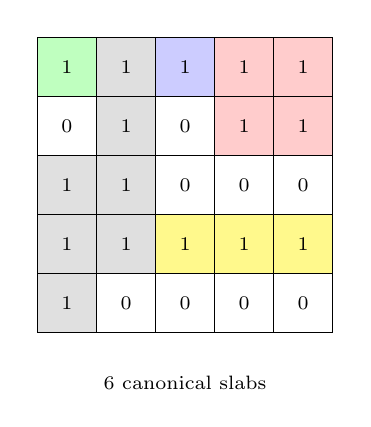
\begin{tikzpicture}[scale=0.7]
\tikzset{cell/.style={minimum size=7.5mm,draw,thin,font=\scriptsize,inner sep=0pt}}
\matrix (m) [matrix of nodes, nodes={cell}, column sep=-\pgflinewidth, row sep=-\pgflinewidth] {
|[fill=green!25]| 1 & |[fill=gray!25]| 1 & |[fill=blue!20]| 1 & |[fill=red!20]| 1 & |[fill=red!20]| 1 \\
0 & |[fill=gray!25]| 1 & 0 & |[fill=red!20]| 1 & |[fill=red!20]| 1 \\
|[fill=black!12]| 1 & |[fill=gray!25]| 1 & 0 & 0 & 0 \\
|[fill=black!12]| 1 & |[fill=gray!25]| 1 & |[fill=yellow!45]| 1 & |[fill=yellow!45]| 1 & |[fill=yellow!45]| 1 \\
|[fill=black!12]| 1 & 0 & 0 & 0 & 0 \\
};
\node[below=3mm,font=\scriptsize] at (m.south) {6 canonical slabs};
\end{tikzpicture}
\end{column}
\end{columns}
\end{frame}

% ============ SLIDE 17 ============
\begin{frame}{Why canonical decomposition is small}
\centering
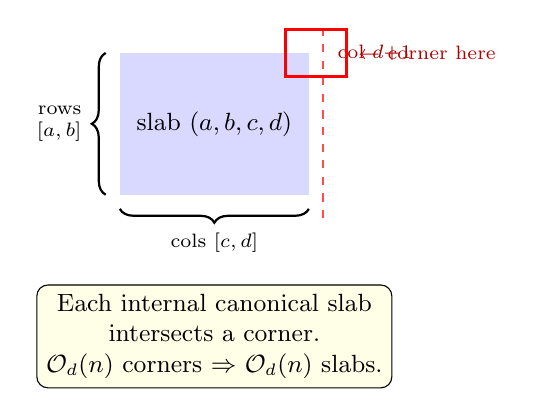
\begin{tikzpicture}[scale=0.6]
% A slab with its boundary probed
\fill[blue!15] (2,1) rectangle (6,4);
\node[font=\small] at (4,2.5) {slab $(a,b,c,d)$};
% Adjacent column
\draw[thick,dashed,red!70] (6.3,0.5) -- (6.3,4.5);
\node[font=\scriptsize,red!60!black,right] at (6.4,4) {col $d{+}1$};

% Corner annotation
\draw[very thick,red] (5.5,3.5) rectangle (6.8,4.5);
\node[font=\scriptsize,red!70!black] at (8.5,4) {$\leftarrow$ corner here};

\draw[decorate,decoration={brace,amplitude=5pt},thick] (1.7,1) -- (1.7,4) node[midway,left=5pt,font=\scriptsize,align=right]{rows\\$[a,b]$};
\draw[decorate,decoration={brace,amplitude=5pt,mirror},thick] (2,0.7) -- (6,0.7) node[midway,below=5pt,font=\scriptsize]{cols $[c,d]$};

\node[draw,rounded corners,fill=yellow!10,font=\small,align=center] at (4,-2) {
Each internal canonical slab\\intersects a corner.\\
$\Oh_d(n)$ corners $\Rightarrow$ $\Oh_d(n)$ slabs.
};
\end{tikzpicture}
\end{frame}

% ============ SLIDE 18 ============
\begin{frame}{Computing canonical decomposition: overview}
\centering
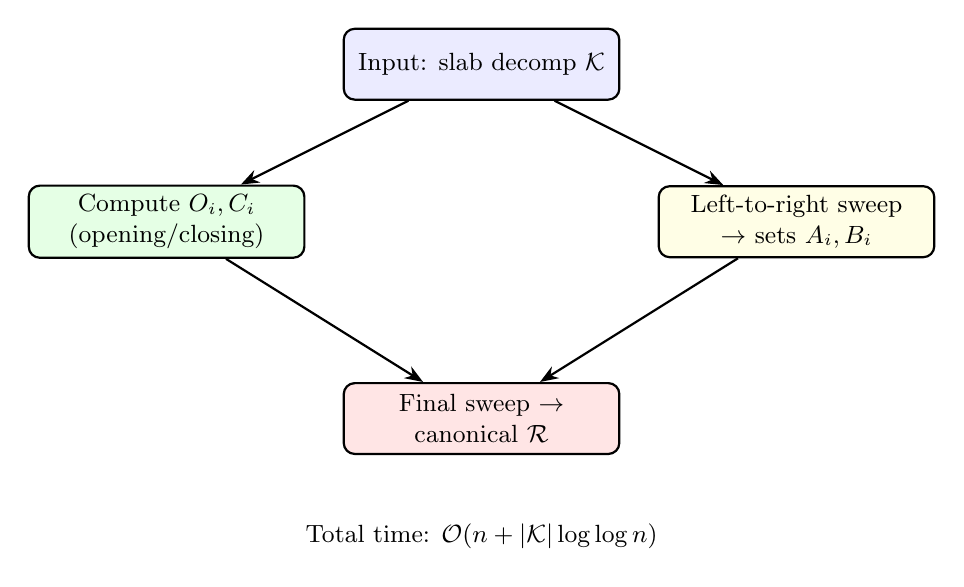
\begin{tikzpicture}[
  block/.style={draw,rounded corners,fill=blue!8,minimum width=3.5cm,minimum height=0.9cm,align=center,font=\small,thick},
  arr/.style={->,>=Stealth,thick}
]
\node[block] (input) at (0,3) {Input: slab decomp $\mathcal{K}$};
\node[block,fill=green!10] (oi) at (-4,1) {Compute $O_i, C_i$\\(opening/closing)};
\node[block,fill=yellow!10] (sweep) at (4,1) {Left-to-right sweep\\$\to$ sets $A_i, B_i$};
\node[block,fill=red!10] (final) at (0,-1.5) {Final sweep $\to$\\canonical $\mathcal{R}$};

\draw[arr] (input) -- (oi);
\draw[arr] (input) -- (sweep);
\draw[arr] (oi) -- (final);
\draw[arr] (sweep) -- (final);

\node[font=\small] at (0,-3) {Total time: $\Oh(n + |\mathcal{K}|\log\log n)$};
\end{tikzpicture}
\end{frame}

% ============ SLIDE 19 ============
\begin{frame}{Sweep: maintaining $\mathtt{strips}_i$}
\centering
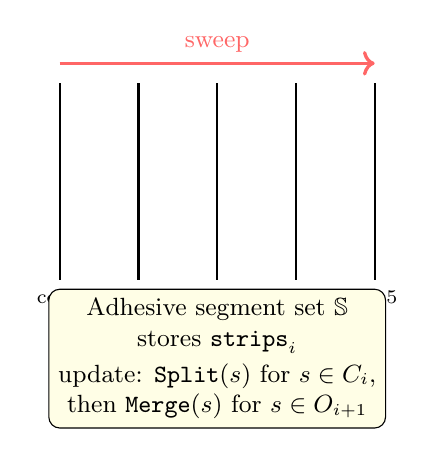
\begin{tikzpicture}[scale=0.5]
% Matrix columns as vertical bars
\foreach \c [count=\i] in {1,...,5} {
  \draw[thick] (\i*2,0) -- (\i*2,5);
  \node[below,font=\scriptsize] at (\i*2,0) {col \i};
}
% Sweep arrow
\draw[->,very thick,red!60] (2,5.5) -- (10,5.5) node[midway,above,font=\small]{sweep};

% Adhesive segment set box
\node[draw,rounded corners,fill=yellow!10,font=\small,align=center] at (6,-2) {
  Adhesive segment set $\mathbb{S}$\\
  stores $\mathtt{strips}_i$\\[2pt]
  update: $\mathtt{Split}(s)$ for $s \in C_i$,\\
  then $\mathtt{Merge}(s)$ for $s \in O_{i+1}$
};
\end{tikzpicture}
\end{frame}

% ============ SLIDE 20 ============
\begin{frame}{Sweep example (from the paper)}
\centering
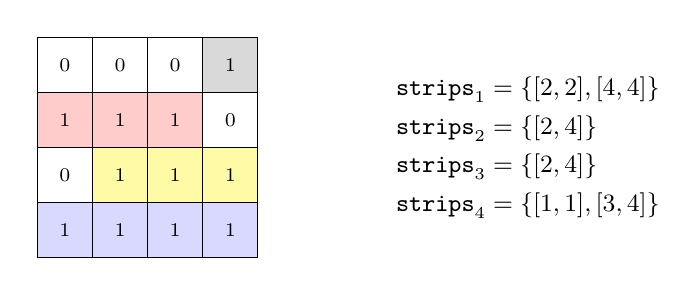
\begin{tikzpicture}[scale=0.6]
\tikzset{cell/.style={minimum size=7mm,draw,thin,font=\scriptsize,inner sep=0pt}}
\matrix (m) [matrix of nodes, nodes={cell}, column sep=-\pgflinewidth, row sep=-\pgflinewidth] {
0 & 0 & 0 & |[fill=black!15]| 1 \\
|[fill=red!20]| 1 & |[fill=red!20]| 1 & |[fill=red!20]| 1 & 0 \\
0 & |[fill=yellow!35]| 1 & |[fill=yellow!35]| 1 & |[fill=yellow!35]| 1 \\
|[fill=blue!15]| 1 & |[fill=blue!15]| 1 & |[fill=blue!15]| 1 & |[fill=blue!15]| 1 \\
};

% Show strips_1
\node[right=15mm,font=\small,align=left] at (m.east) {
  $\mathtt{strips}_1 = \{[2,2],[4,4]\}$\\[3pt]
  $\mathtt{strips}_2 = \{[2,4]\}$\\[3pt]
  $\mathtt{strips}_3 = \{[2,4]\}$\\[3pt]
  $\mathtt{strips}_4 = \{[1,1],[3,4]\}$
};
\end{tikzpicture}
\end{frame}

% ============ SLIDE 21 ============
\begin{frame}{Final sweep: pairing $A_i$ and $B_i$}
\centering
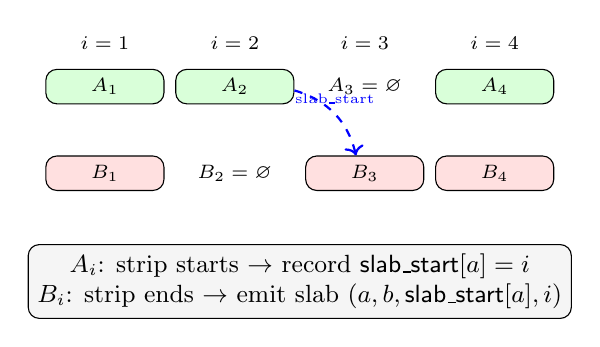
\begin{tikzpicture}[scale=0.55]
\foreach \i in {1,...,4} {
  \node[font=\scriptsize] at (\i*3, 3) {$i=\i$};
}
% A_i arrows down
\node[draw,fill=green!15,font=\scriptsize,rounded corners,minimum width=1.5cm] (a1) at (3,2) {$A_1$};
\node[draw,fill=green!15,font=\scriptsize,rounded corners,minimum width=1.5cm] (a2) at (6,2) {$A_2$};
\node[font=\scriptsize] at (9,2) {$A_3=\varnothing$};
\node[draw,fill=green!15,font=\scriptsize,rounded corners,minimum width=1.5cm] (a4) at (12,2) {$A_4$};

\node[draw,fill=red!12,font=\scriptsize,rounded corners,minimum width=1.5cm] (b1) at (3,0) {$B_1$};
\node[font=\scriptsize] at (6,0) {$B_2=\varnothing$};
\node[draw,fill=red!12,font=\scriptsize,rounded corners,minimum width=1.5cm] (b3) at (9,0) {$B_3$};
\node[draw,fill=red!12,font=\scriptsize,rounded corners,minimum width=1.5cm] (b4) at (12,0) {$B_4$};

% slab_start logic
\draw[->,thick,dashed,blue] (a2) to[bend left=30] node[above,font=\tiny]{slab\_start} (b3);

\node[draw,rounded corners,fill=gray!8,font=\small,align=center] at (7.5,-2.5) {
  $A_i$: strip starts $\to$ record $\mathsf{slab\_start}[a]=i$\\
  $B_i$: strip ends $\to$ emit slab $(a,b,\mathsf{slab\_start}[a],i)$
};
\end{tikzpicture}
\end{frame}

% ============ SLIDE 22 ============
\begin{frame}{Amortized data structure: architecture}
\centering
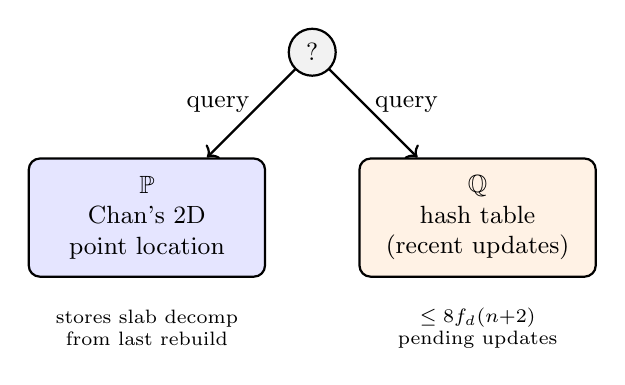
\begin{tikzpicture}[scale=0.7,
  box/.style={draw,thick,rounded corners,minimum width=3cm,minimum height=1.5cm,align=center,font=\small}
]
\node[box,fill=blue!10] (P) at (0,0) {$\mathbb{P}$\\Chan's 2D\\point location};
\node[box,fill=orange!10] (Q) at (6,0) {$\mathbb{Q}$\\hash table\\(recent updates)};

\draw[->,thick] (3,3) -- node[left,font=\small]{query} (P);
\draw[->,thick] (3,3) -- node[right,font=\small]{query} (Q);
\node[draw,circle,thick,fill=gray!10,font=\small] at (3,3) {?};

\node[font=\scriptsize,align=center] at (0,-2) {stores slab decomp\\from last rebuild};
\node[font=\scriptsize,align=center] at (6,-2) {$\leq 8f_d(n{+}2)$\\pending updates};
\end{tikzpicture}
\end{frame}

% ============ SLIDE 23 ============
\begin{frame}{Query: check $\mathbb{Q}$ then $\mathbb{P}$}
\centering
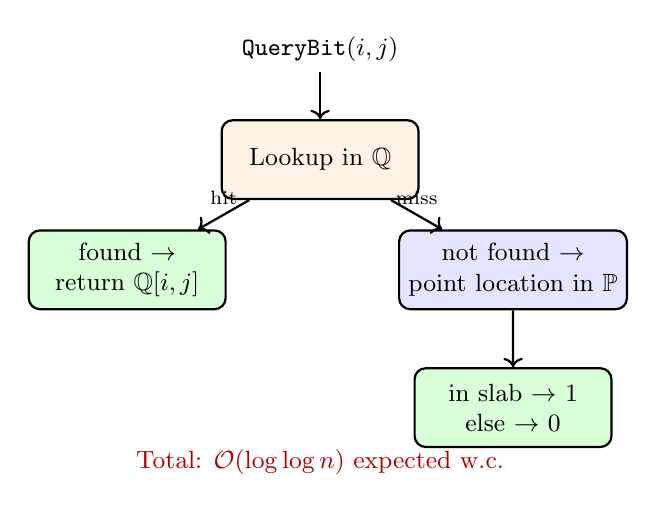
\begin{tikzpicture}[scale=0.7,
  box/.style={draw,thick,rounded corners,minimum width=2.5cm,minimum height=1cm,align=center,font=\small}
]
\node[font=\small] (query) at (0,3) {$\mathtt{QueryBit}(i,j)$};
\node[box,fill=orange!10] (Q) at (0,1) {Lookup in $\mathbb{Q}$};
\node[box,fill=green!15] (hit) at (-3.5,-1) {found $\to$\\return $\mathbb{Q}[i,j]$};
\node[box,fill=blue!10] (P) at (3.5,-1) {not found $\to$\\point location in $\mathbb{P}$};
\node[box,fill=green!15] (res) at (3.5,-3.5) {in slab $\to$ 1\\else $\to$ 0};

\draw[->,thick] (query) -- (Q);
\draw[->,thick] (Q) -- node[above,font=\scriptsize]{hit} (hit);
\draw[->,thick] (Q) -- node[above,font=\scriptsize]{miss} (P);
\draw[->,thick] (P) -- (res);

\node[font=\small,red!70!black] at (0,-4.5) {Total: $\Oh(\log\log n)$ expected w.c.};
\end{tikzpicture}
\end{frame}

% ============ SLIDE 24 ============
\begin{frame}{Update and rebuild trigger}
\centering
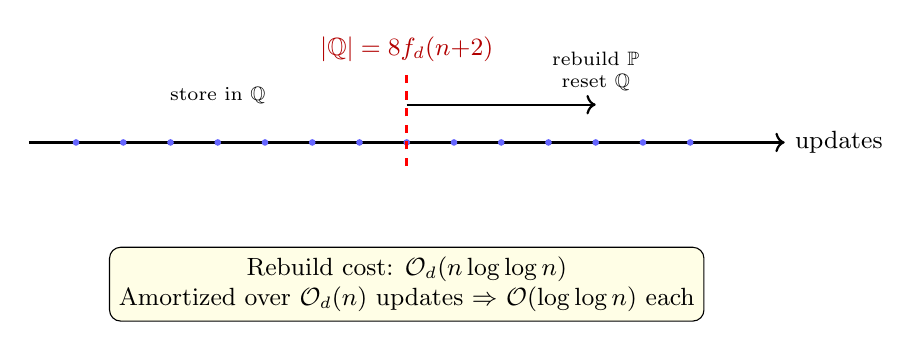
\begin{tikzpicture}[scale=0.6]
% Timeline of updates
\draw[thick,->] (0,0) -- (16,0) node[right,font=\small]{updates};
\foreach \x in {1,...,14} {
  \fill[blue!60] (\x,0) circle (2pt);
}
% Threshold
\draw[very thick,red,dashed] (8,-.5) -- (8,1.5);
\node[above,font=\small,red!70!black] at (8,1.5) {$|\mathbb{Q}| = 8f_d(n{+}2)$};
\node[font=\scriptsize] at (4,1) {store in $\mathbb{Q}$};
\node[font=\scriptsize,align=center] at (12,1.5) {rebuild $\mathbb{P}$\\reset $\mathbb{Q}$};
\draw[->,thick] (8,0.8) -- (12,0.8);

\node[draw,rounded corners,fill=yellow!10,font=\small,align=center] at (8,-3) {
  Rebuild cost: $\Oh_d(n\log\log n)$\\
  Amortized over $\Oh_d(n)$ updates $\Rightarrow$ $\Oh(\log\log n)$ each
};
\end{tikzpicture}
\end{frame}

% ============ SLIDE 25 ============
\begin{frame}{Rebuild: splitting slabs by 0-updates}
\centering
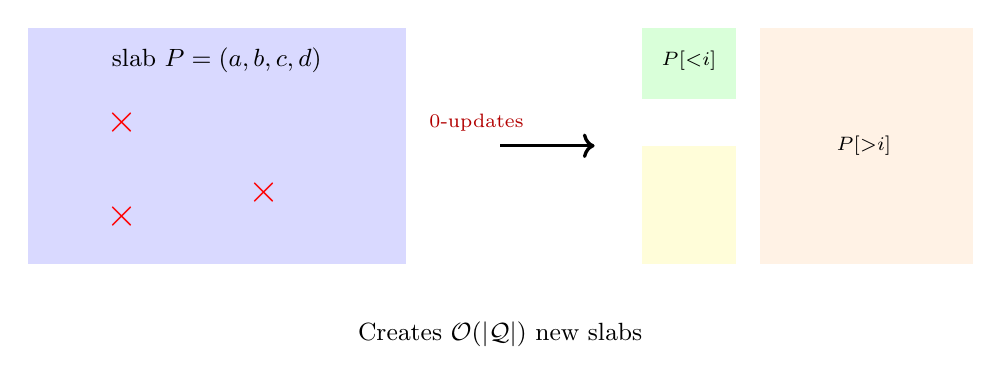
\begin{tikzpicture}[scale=0.6]
% Original slab
\fill[blue!15] (0,0) rectangle (8,5);
\node[font=\small] at (4,4.3) {slab $P=(a,b,c,d)$};
% 0-updates as crosses
\node[font=\Large,red] at (2,3) {$\times$};
\node[font=\Large,red] at (5,1.5) {$\times$};
\node[font=\Large,red] at (2,1) {$\times$};
\node[font=\scriptsize,red!70!black] at (9.5,3) {0-updates};

\draw[->,very thick] (10,2.5) -- (12,2.5);

% Split result
\fill[green!15] (13,3.5) rectangle (15,5);
\fill[yellow!15] (13,0) rectangle (15,2.5);
\fill[orange!10] (15.5,0) rectangle (20,5);
\node[font=\scriptsize] at (14,4.3) {$P[{<}i]$};
\node[font=\scriptsize] at (17.7,2.5) {$P[{>}i]$};

\node[font=\small] at (10,-1.5) {Creates $\Oh(|\mathcal{Q}|)$ new slabs};
\end{tikzpicture}
\end{frame}

% ============ SLIDE 26 ============
\begin{frame}{De-amortization: epoch structure}
\centering
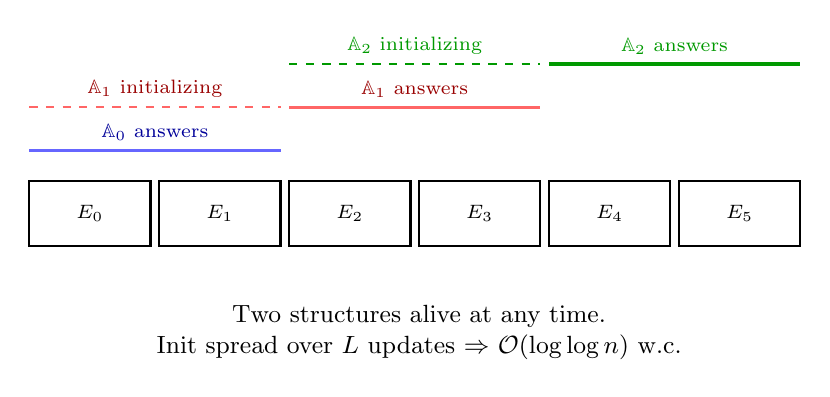
\begin{tikzpicture}[scale=0.55]
% Epochs
\foreach \i [evaluate=\i as \x using \i*3] in {0,...,5} {
  \draw[thick] (\x,0) rectangle (\x+2.8,1.5);
  \node[font=\scriptsize] at (\x+1.4,0.75) {$E_\i$};
}
% A_0 lifetime
\draw[very thick,blue!60] (0,2.2) -- (5.8,2.2);
\node[font=\scriptsize,blue!60!black,above] at (2.9,2.2) {$\mathbb{A}_0$ answers};

% A_1 init + active
\draw[thick,dashed,red!60] (0,3.2) -- (5.8,3.2);
\node[font=\scriptsize,red!60!black,above] at (2.9,3.2) {$\mathbb{A}_1$ initializing};
\draw[very thick,red!60] (6,3.2) -- (11.8,3.2);
\node[font=\scriptsize,red!60!black,above] at (8.9,3.2) {$\mathbb{A}_1$ answers};

% A_2 init + active
\draw[thick,dashed,green!60!black] (6,4.2) -- (11.8,4.2);
\node[font=\scriptsize,green!60!black,above] at (8.9,4.2) {$\mathbb{A}_2$ initializing};
\draw[very thick,green!60!black] (12,4.2) -- (17.8,4.2);
\node[font=\scriptsize,green!60!black,above] at (14.9,4.2) {$\mathbb{A}_2$ answers};

\node[font=\small,align=center] at (9,-2) {Two structures alive at any time.\\
Init spread over $L$ updates $\Rightarrow$ $\Oh(\log\log n)$ w.c.};
\end{tikzpicture}
\end{frame}

% ============ SLIDE 27 ============
\begin{frame}{De-amortization: catch-up phase}
\centering
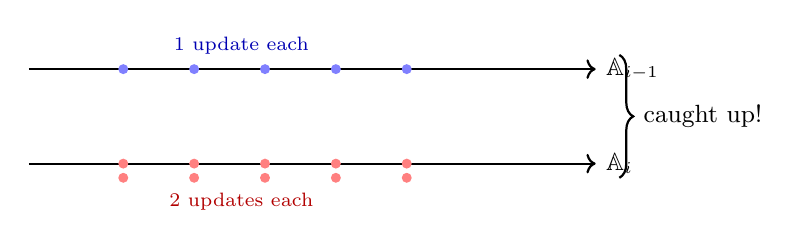
\begin{tikzpicture}[scale=0.6]
% Two parallel timelines
\draw[thick,->] (0,2) -- (12,2) node[right,font=\small]{$\mathbb{A}_{i-1}$};
\draw[thick,->] (0,0) -- (12,0) node[right,font=\small]{$\mathbb{A}_{i}$};

% Updates on A_{i-1}
\foreach \x in {1,...,5} {
  \fill[blue!50] (\x*1.5+0.5,2) circle (3pt);
}
\node[font=\scriptsize,blue!70!black] at (4.5,2.5) {1 update each};

% Double updates on A_i
\foreach \x in {1,...,5} {
  \fill[red!50] (\x*1.5+0.5,0) circle (3pt);
  \fill[red!50] (\x*1.5+0.5,-0.3) circle (3pt);
}
\node[font=\scriptsize,red!70!black] at (4.5,-0.8) {2 updates each};

\draw[decorate,decoration={brace,amplitude=5pt},thick] (12.5,2.3) -- (12.5,-0.3) node[midway,right=5pt,font=\small]{caught up!};
\end{tikzpicture}
\end{frame}

% ============ SLIDE 28 ============
\begin{frame}{De-amortization: the snapshot trick}
\centering
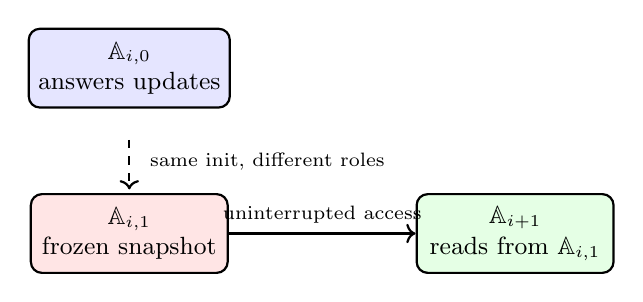
\begin{tikzpicture}[scale=0.7,
  box/.style={draw,thick,rounded corners,minimum width=2.5cm,minimum height=1cm,align=center,font=\small}
]
\node[box,fill=blue!10] (a0) at (0,2) {$\mathbb{A}_{i,0}$\\answers updates};
\node[box,fill=red!10] (a1) at (0,-1) {$\mathbb{A}_{i,1}$\\frozen snapshot};
\node[box,fill=green!10] (next) at (7,-1) {$\mathbb{A}_{i+1}$\\reads from $\mathbb{A}_{i,1}$};

\draw[->,thick] (a1) -- node[above,font=\scriptsize]{uninterrupted access} (next);
\draw[->,thick,dashed] (0,0.7) -- (0,-0.2);
\node[font=\scriptsize,right] at (0.2,0.3) {same init, different roles};
\end{tikzpicture}

\medskip
Two copies ensure one can serve queries while the other lends data.
\end{frame}

% ============ SLIDE 29 ============
\begin{frame}{Summary}
\centering
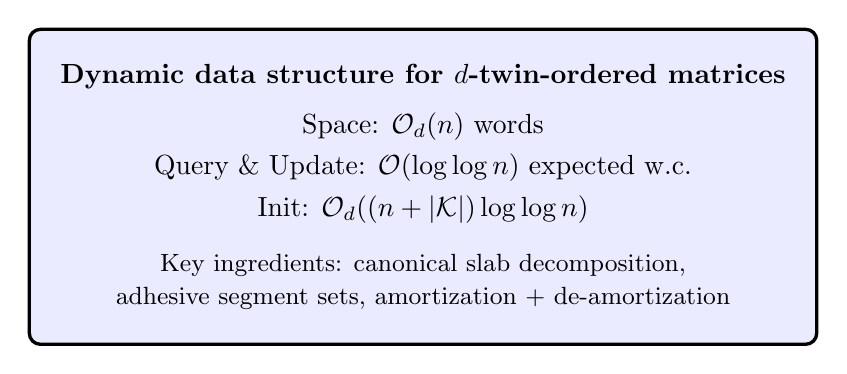
\begin{tikzpicture}[scale=0.6]
\node[draw,very thick,rounded corners,fill=blue!8,minimum width=10cm,minimum height=4cm,align=center,font=\normalsize] at (0,0) {
  \textbf{Dynamic data structure for $d$-twin-ordered matrices}\\[6pt]
  Space: $\Oh_d(n)$ words\\[3pt]
  Query \& Update: $\Oh(\log\log n)$ expected w.c.\\[3pt]
  Init: $\Oh_d((n+|\mathcal{K}|)\log\log n)$\\[8pt]
  {\small Key ingredients: canonical slab decomposition,}\\
  {\small adhesive segment sets, amortization + de-amortization}
};
\end{tikzpicture}
\end{frame}

% ============ SLIDE 30 ============
\begin{frame}{Thank you!}
\centering
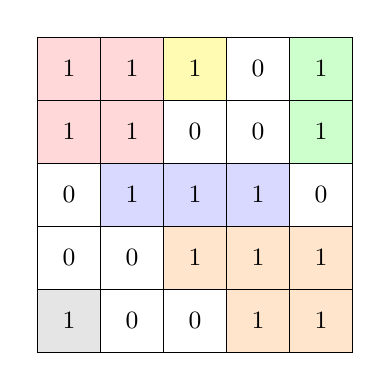
\begin{tikzpicture}[scale=0.6]
\matrix[matrix of nodes, nodes={minimum size=8mm, draw, thin, font=\small},
  column sep=-\pgflinewidth, row sep=-\pgflinewidth]{
|[fill=red!15]| 1 & |[fill=red!15]| 1 & |[fill=yellow!30]| 1 & 0 & |[fill=green!20]| 1 \\
|[fill=red!15]| 1 & |[fill=red!15]| 1 & 0 & 0 & |[fill=green!20]| 1 \\
0 & |[fill=blue!15]| 1 & |[fill=blue!15]| 1 & |[fill=blue!15]| 1 & 0 \\
0 & 0 & |[fill=orange!20]| 1 & |[fill=orange!20]| 1 & |[fill=orange!20]| 1 \\
|[fill=gray!20]| 1 & 0 & 0 & |[fill=orange!20]| 1 & |[fill=orange!20]| 1 \\
};
\end{tikzpicture}

\bigskip
{\Large Questions?}

\bigskip
{\small Contact: \texttt{\{j.czyzewska, w.nadara, michal.pilipczuk, anka\}@mimuw.edu.pl}}
\end{frame}

% ======== BACKUP SLIDES ========

\appendix
\begin{frame}[noframenumbering]{Backup: Chan's static 2D point location}
\centering
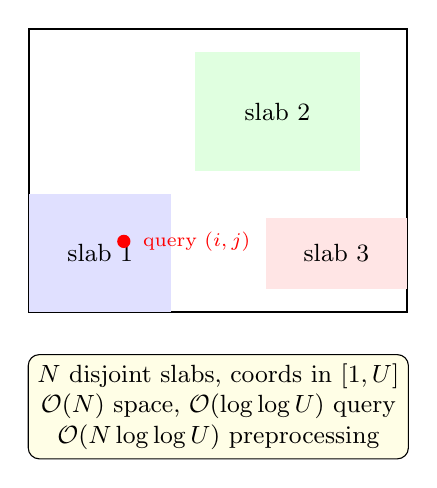
\begin{tikzpicture}[scale=0.6]
\draw[thick] (0,0) rectangle (8,6);
\fill[blue!12] (0,0) rectangle (3,2.5);
\fill[green!12] (3.5,3) rectangle (7,5.5);
\fill[red!10] (5,0.5) rectangle (8,2);
\node[font=\small] at (1.5,1.25) {slab 1};
\node[font=\small] at (5.25,4.25) {slab 2};
\node[font=\small] at (6.5,1.25) {slab 3};
% Query point
\fill[red] (2,1.5) circle (4pt);
\node[font=\scriptsize,red,right] at (2.2,1.5) {query $(i,j)$};
\node[draw,rounded corners,fill=yellow!10,font=\small,align=center] at (4,-2) {
  $N$ disjoint slabs, coords in $[1,U]$\\
  $\Oh(N)$ space, $\Oh(\log\log U)$ query\\
  $\Oh(N\log\log U)$ preprocessing
};
\end{tikzpicture}
\end{frame}

\begin{frame}[noframenumbering]{Backup: Rebuild procedure in detail}
\centering
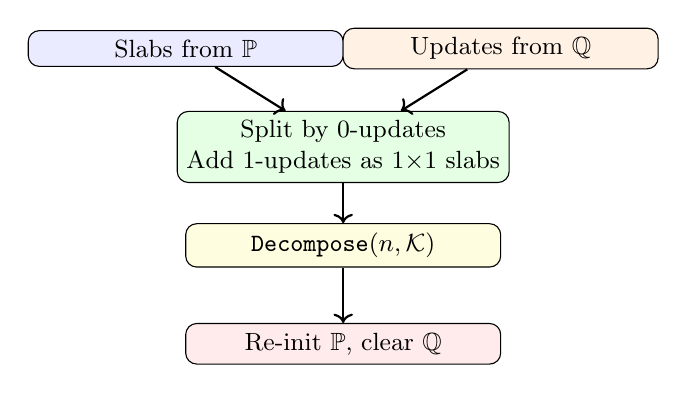
\begin{tikzpicture}[scale=0.5]
\node[draw,rounded corners,fill=blue!8,align=center,font=\small,minimum width=4cm] (slabs) at (0,4) {Slabs from $\mathbb{P}$};
\node[draw,rounded corners,fill=orange!10,align=center,font=\small,minimum width=4cm] (updates) at (8,4) {Updates from $\mathbb{Q}$};
\node[draw,rounded corners,fill=green!10,align=center,font=\small,minimum width=4cm] (split) at (4,1.5) {Split by 0-updates\\Add 1-updates as $1{\times}1$ slabs};
\node[draw,rounded corners,fill=yellow!12,align=center,font=\small,minimum width=4cm] (decompose) at (4,-1) {$\mathtt{Decompose}(n,\mathcal{K})$};
\node[draw,rounded corners,fill=red!8,align=center,font=\small,minimum width=4cm] (reinit) at (4,-3.5) {Re-init $\mathbb{P}$, clear $\mathbb{Q}$};

\draw[->,thick] (slabs) -- (split);
\draw[->,thick] (updates) -- (split);
\draw[->,thick] (split) -- (decompose);
\draw[->,thick] (decompose) -- (reinit);
\end{tikzpicture}
\end{frame}

\begin{frame}[noframenumbering]{Backup: Adhesive segment set implementation}
\centering
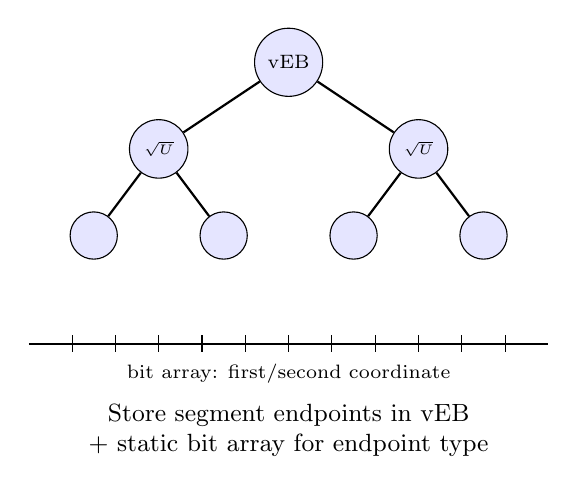
\begin{tikzpicture}[scale=0.55]
% vEB tree sketch
\node[draw,circle,fill=blue!10,minimum size=8mm,font=\scriptsize] (root) at (6,5) {vEB};
\node[draw,circle,fill=blue!10,minimum size=7mm,font=\tiny] (l) at (3,3) {$\sqrt{U}$};
\node[draw,circle,fill=blue!10,minimum size=7mm,font=\tiny] (r) at (9,3) {$\sqrt{U}$};
\node[draw,circle,fill=blue!10,minimum size=6mm,font=\tiny] (ll) at (1.5,1) {};
\node[draw,circle,fill=blue!10,minimum size=6mm,font=\tiny] (lr) at (4.5,1) {};
\node[draw,circle,fill=blue!10,minimum size=6mm,font=\tiny] (rl) at (7.5,1) {};
\node[draw,circle,fill=blue!10,minimum size=6mm,font=\tiny] (rr) at (10.5,1) {};
\draw[thick] (root) -- (l); \draw[thick] (root) -- (r);
\draw[thick] (l) -- (ll); \draw[thick] (l) -- (lr);
\draw[thick] (r) -- (rl); \draw[thick] (r) -- (rr);

% Extra bit array
\draw[thick] (0,-1.5) -- (12,-1.5);
\foreach \x in {1,...,11} {
  \draw (\x,-1.3) -- (\x,-1.7);
}
\node[font=\scriptsize] at (6,-2.2) {bit array: first/second coordinate};
\node[font=\small,align=center] at (6,-3.5) {Store segment endpoints in vEB\\+ static bit array for endpoint type};
\end{tikzpicture}
\end{frame}

\end{document}
